
%(BEGIN_QUESTION)
% Copyright 2010, Tony R. Kuphaldt, released under the Creative Commons Attribution License (v 1.0)
% This means you may do almost anything with this work of mine, so long as you give me proper credit

How much water (at 60$^{o}$ F) will flow through this valve when wide open?

$$\includegraphics[width=15.5cm]{i01373x01.eps}$$

Now suppose the valve is closed off until its $C_v$ = 4 instead of 8.  Assuming the same upstream and downstream pressures, what will the new flow rate be?  Does the flow rate follow $C_v$ linearly, or not?  Why is this?

\vskip 20pt \vbox{\hrule \hbox{\strut \vrule{} {\bf Suggestions for Socratic discussion} \vrule} \hrule}

\begin{itemize}
\item{} How realistic do you think it is to assume the same upstream and downstream pressures when the valve moves to a different stem position?  Do you think those pressures would remain the same for all valve positions in a realistic scenario?  Why or why not?
\item{} What type of control valve and actuator are used in this application?
\end{itemize}

\underbar{file i01373}
%(END_QUESTION)





%(BEGIN_ANSWER)

$Q$ = 52.46 GPM at $C_v$ = 8
 
\vskip 10pt

$Q$ = 26.23 GPM at $C_v$ = 4

%(END_ANSWER)





%(BEGIN_NOTES)


%INDEX% Final Control Elements, valve: sizing

%(END_NOTES)


